\documentclass{beamer}
\usepackage[T1]{fontenc}
\usepackage[utf8]{inputenc}
\usepackage[polish]{babel}
\usepackage{lmodern}
\usepackage{graphicx}
\usepackage{hyperref}

\title{Analiza partii szachowych o mistrzostwo świata}
\author{Bartek Grabowski \\ Witold Winiarski}
\date{\today}

\begin{document}

\frame{\titlepage}

\begin{frame}{Spis treści}
  \tableofcontents
\end{frame}

\section{Najpopularniejsze otwarcia}
\begin{frame}{Top 20 otwarć w partiach o mistrzostwo świata}
  \begin{center}
    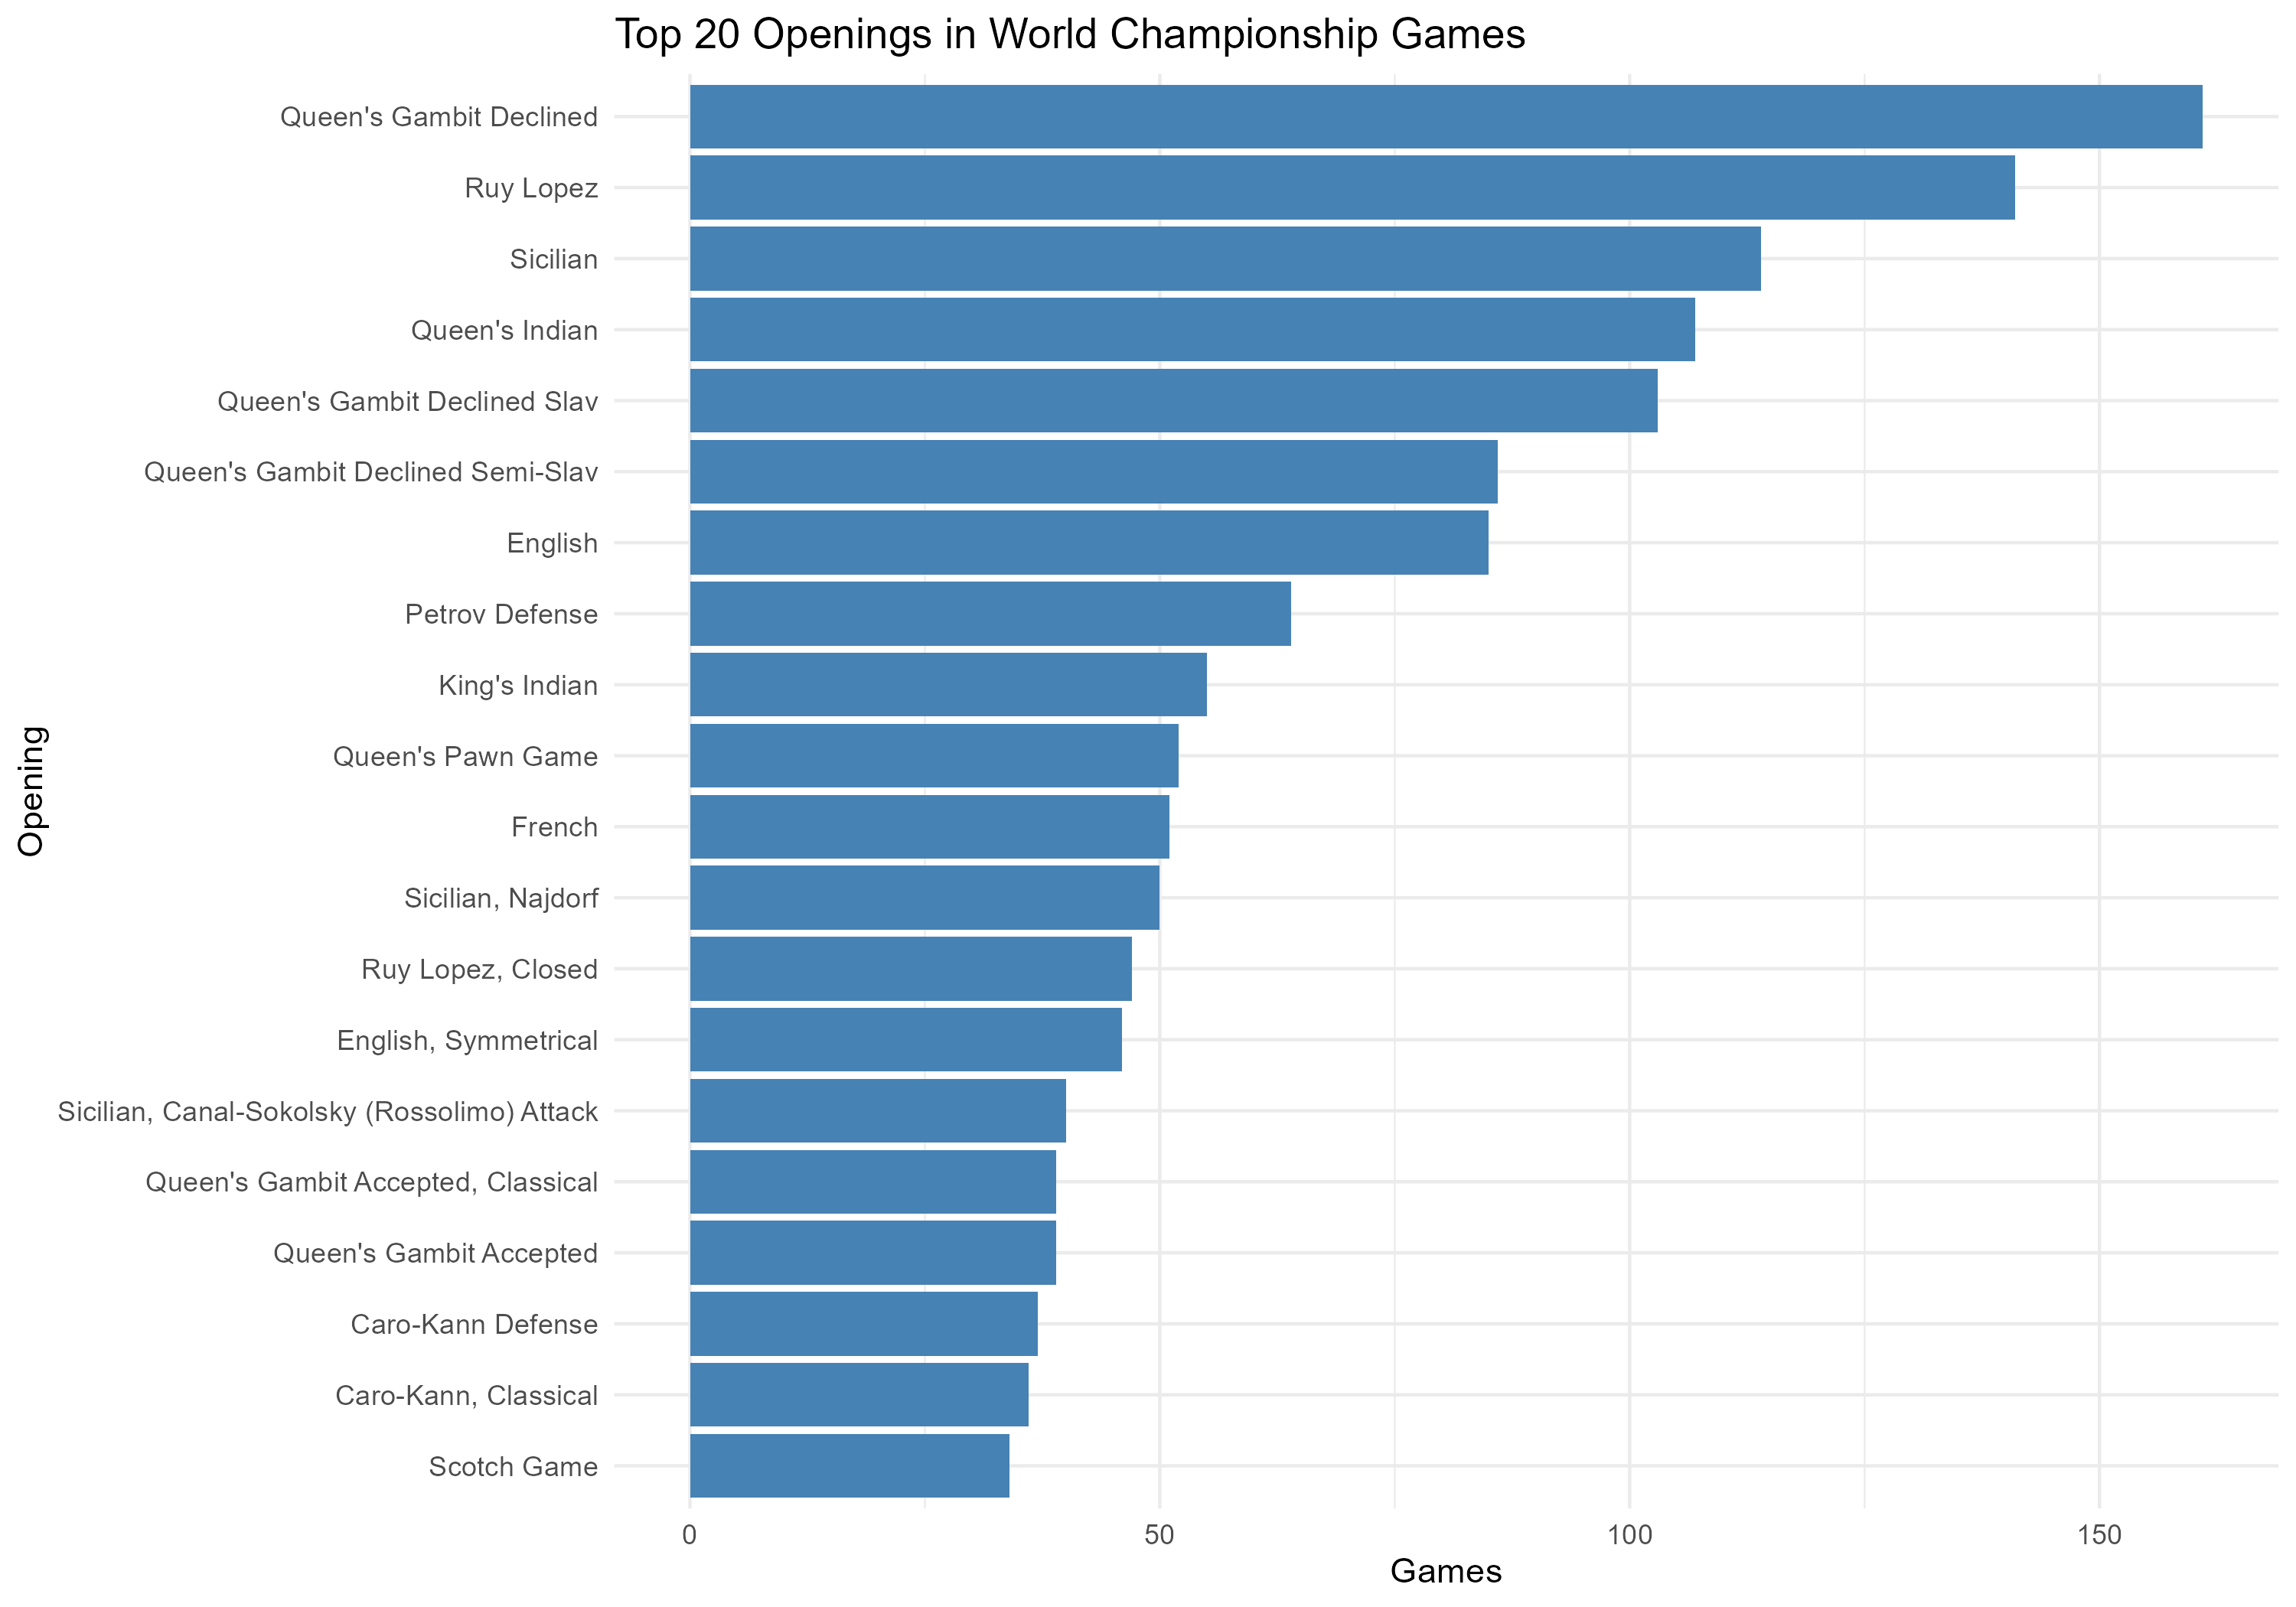
\includegraphics[width=0.9\textwidth]{../../ChessPlots/openings_top20.png}
  \end{center}
  \small
  Najczęściej wybierane otwarcia w historii meczów o mistrzostwo świata.
\end{frame}

\section{Wyniki partii}
\begin{frame}{Rozkład wyników partii}
  \begin{center}
    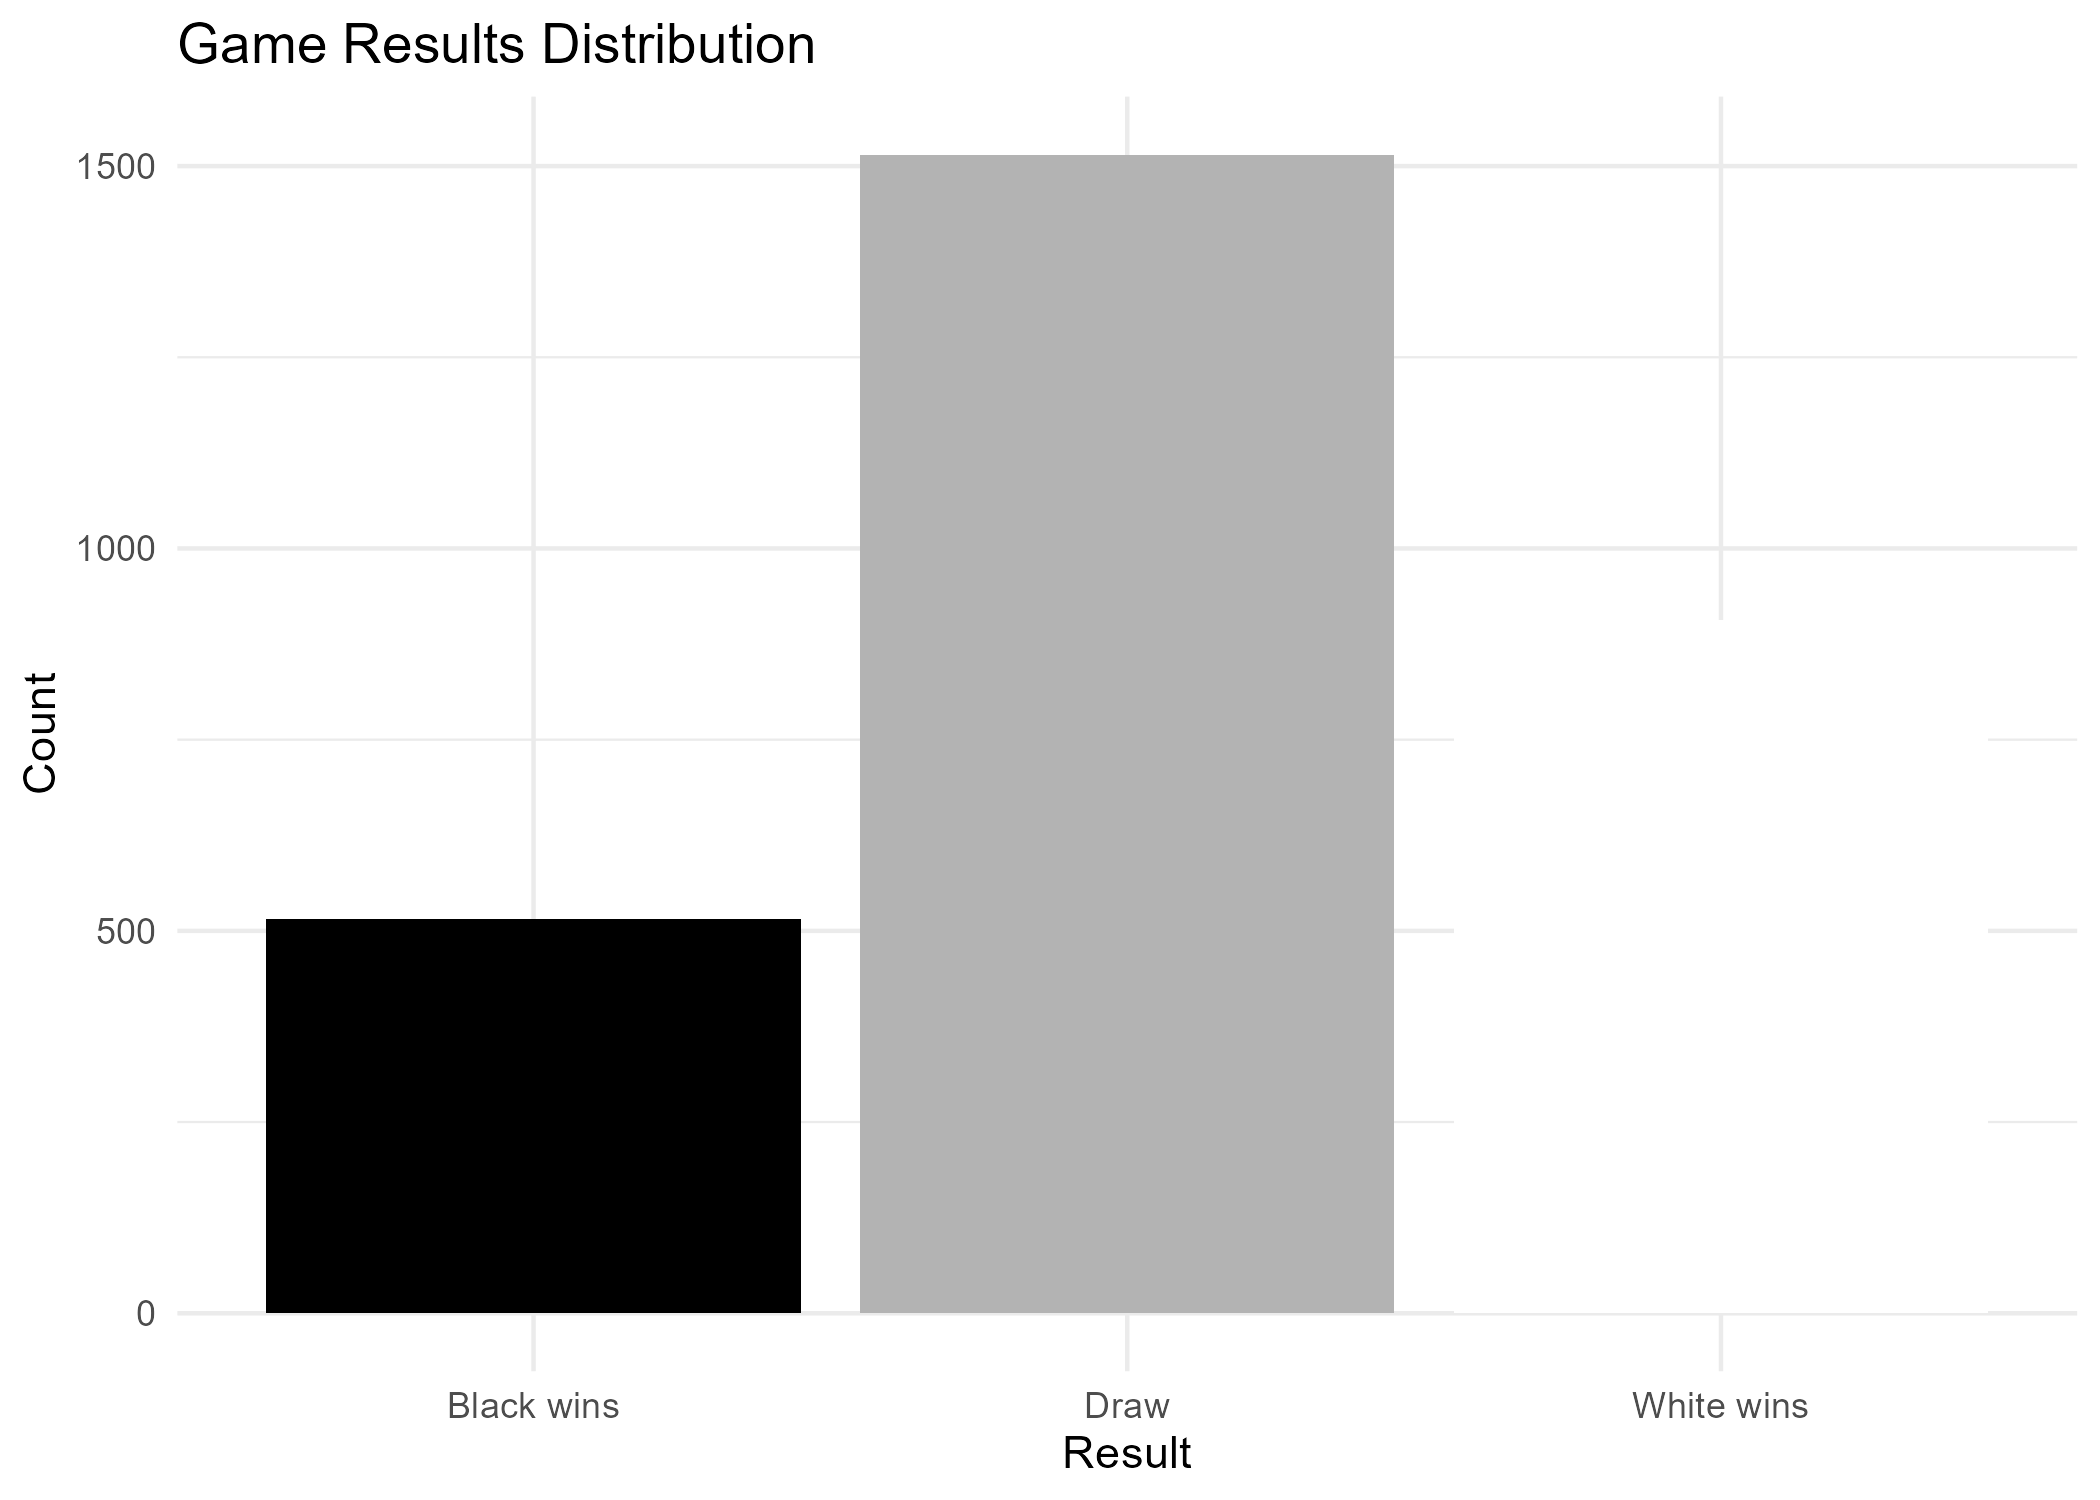
\includegraphics[width=0.7\textwidth]{../../ChessPlots/results_distribution.png}
  \end{center}
  \small
  Procentowy udział zwycięstw białych, czarnych oraz remisów.
\end{frame}

\section{Różnice rankingowe}
\begin{frame}{Rozkład różnic rankingowych ELO}
  \begin{center}
    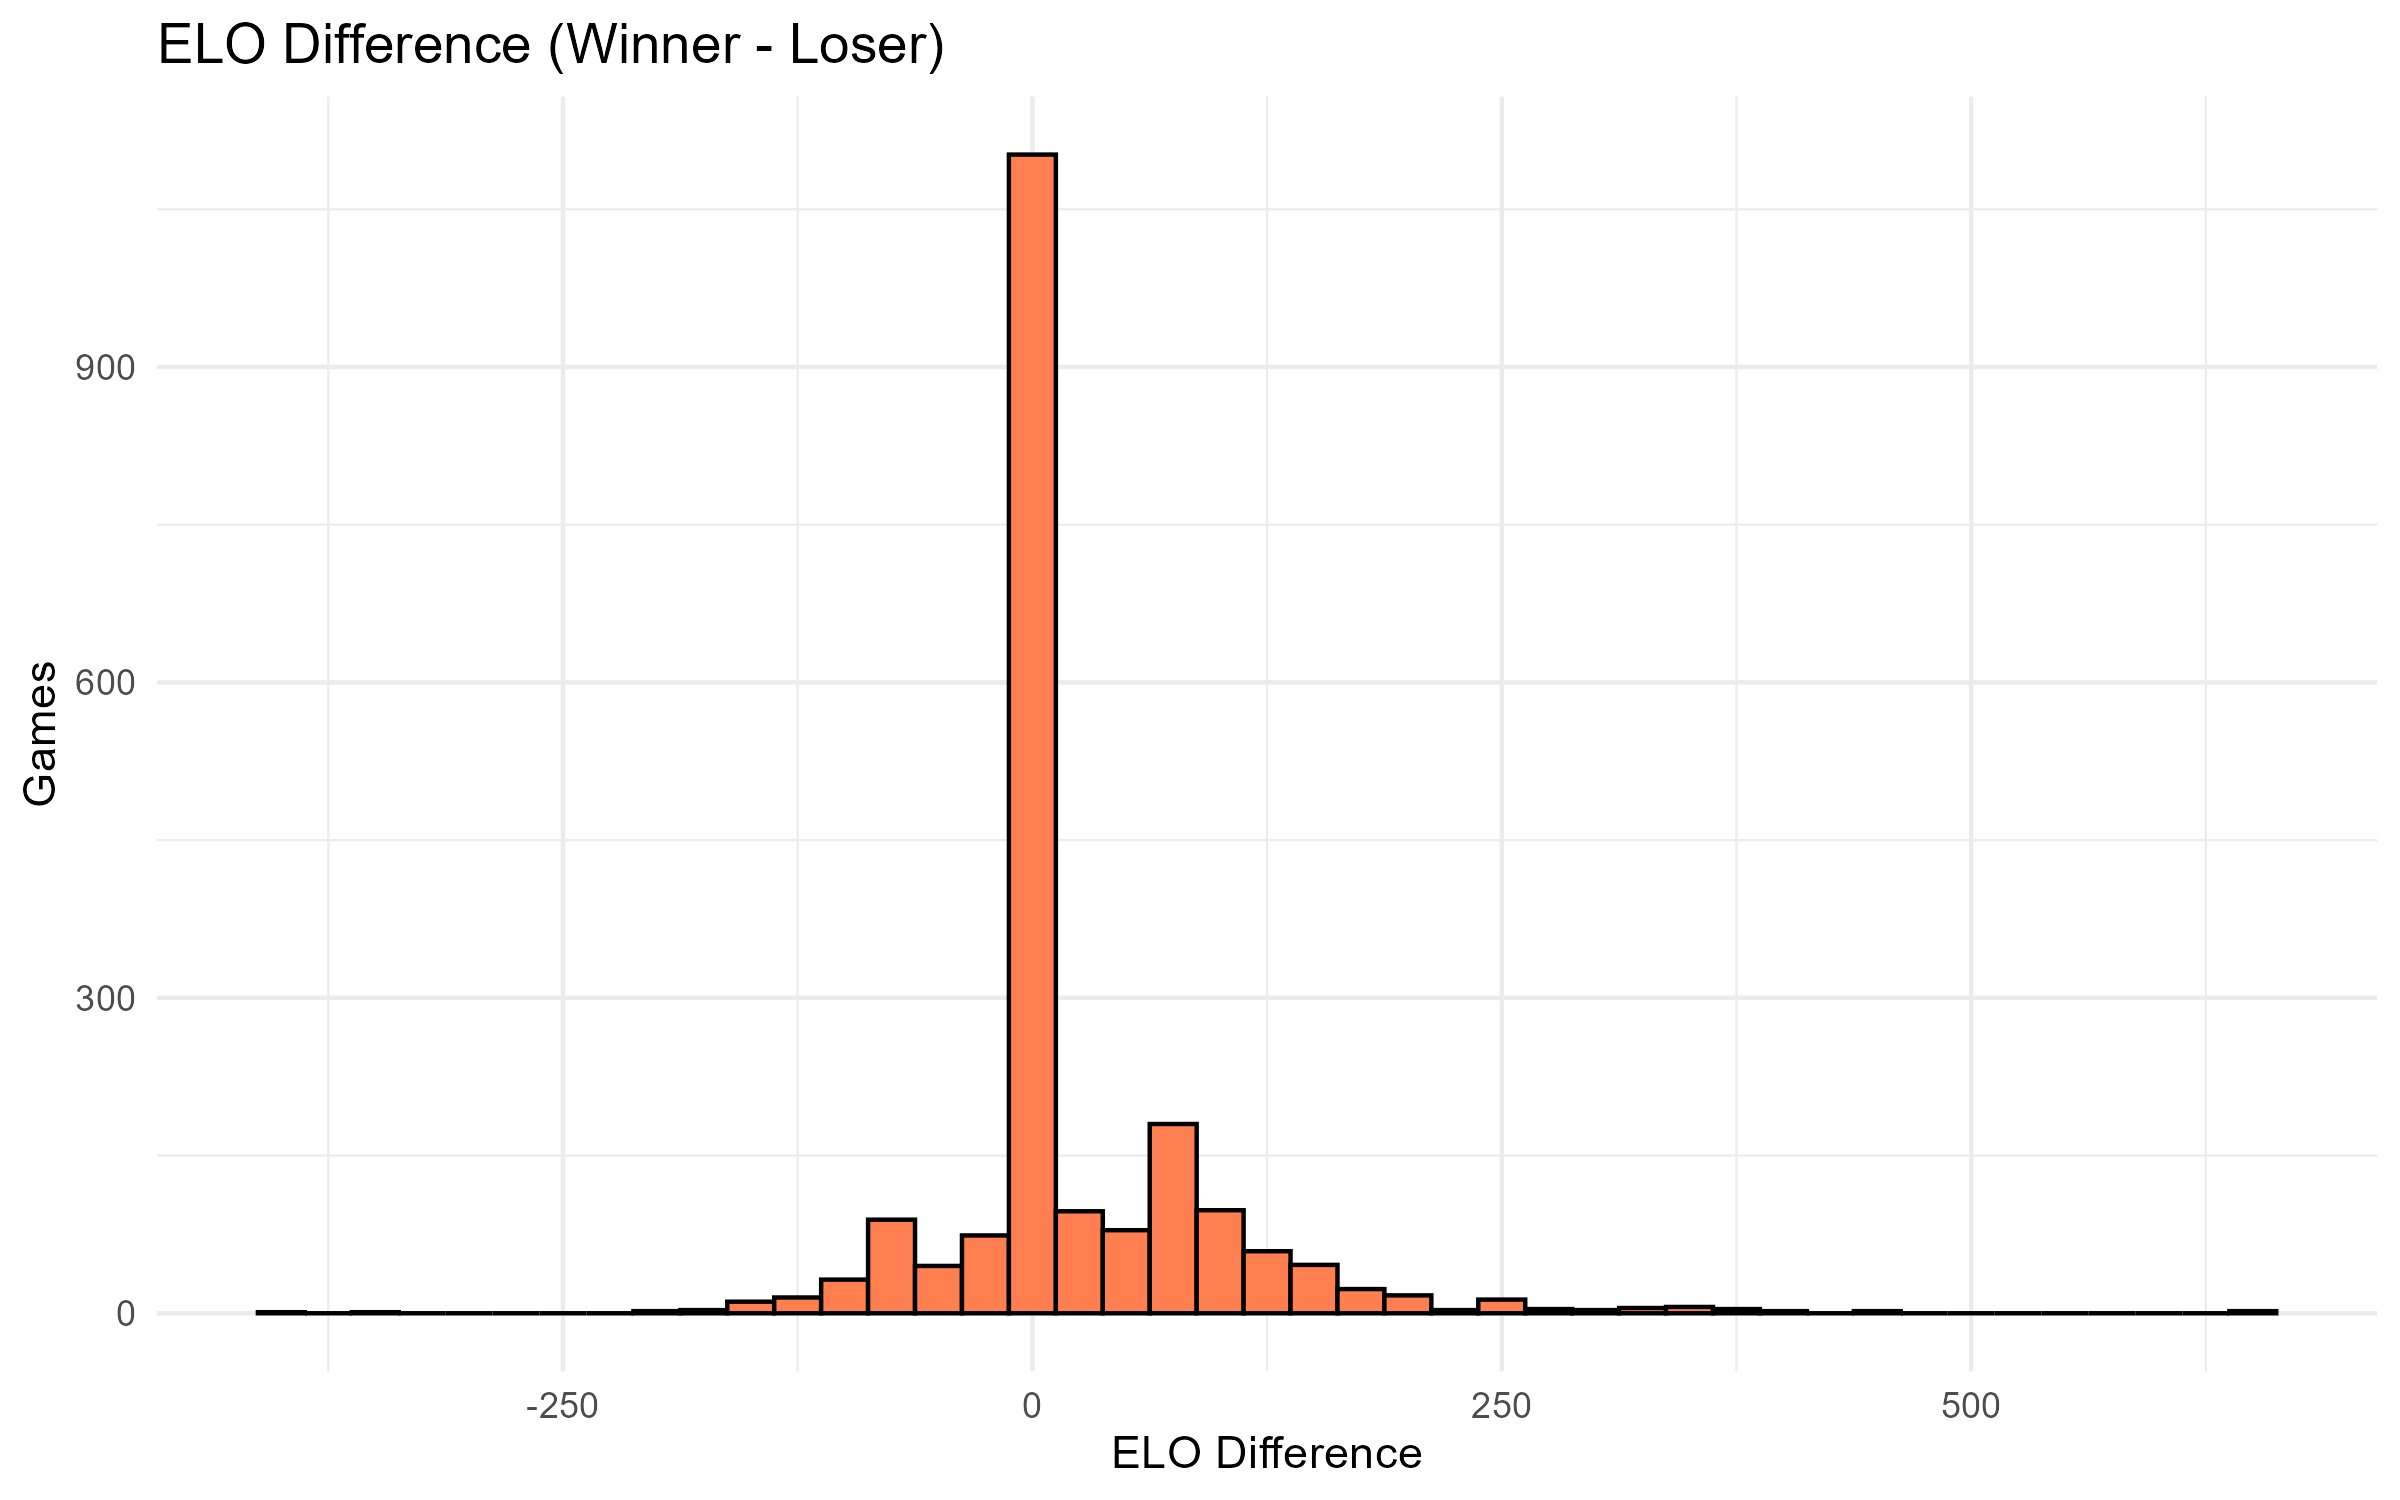
\includegraphics[width=0.8\textwidth]{../../ChessPlots/elo_diff_hist.png}
  \end{center}
  \small
  Histogram różnic rankingowych (ELO) pomiędzy zwycięzcą a przegranym.
\end{frame}

\section{Otwarcia a wyniki}
\begin{frame}{Wyniki według otwarć (min. 10 partii)}
  \begin{center}
    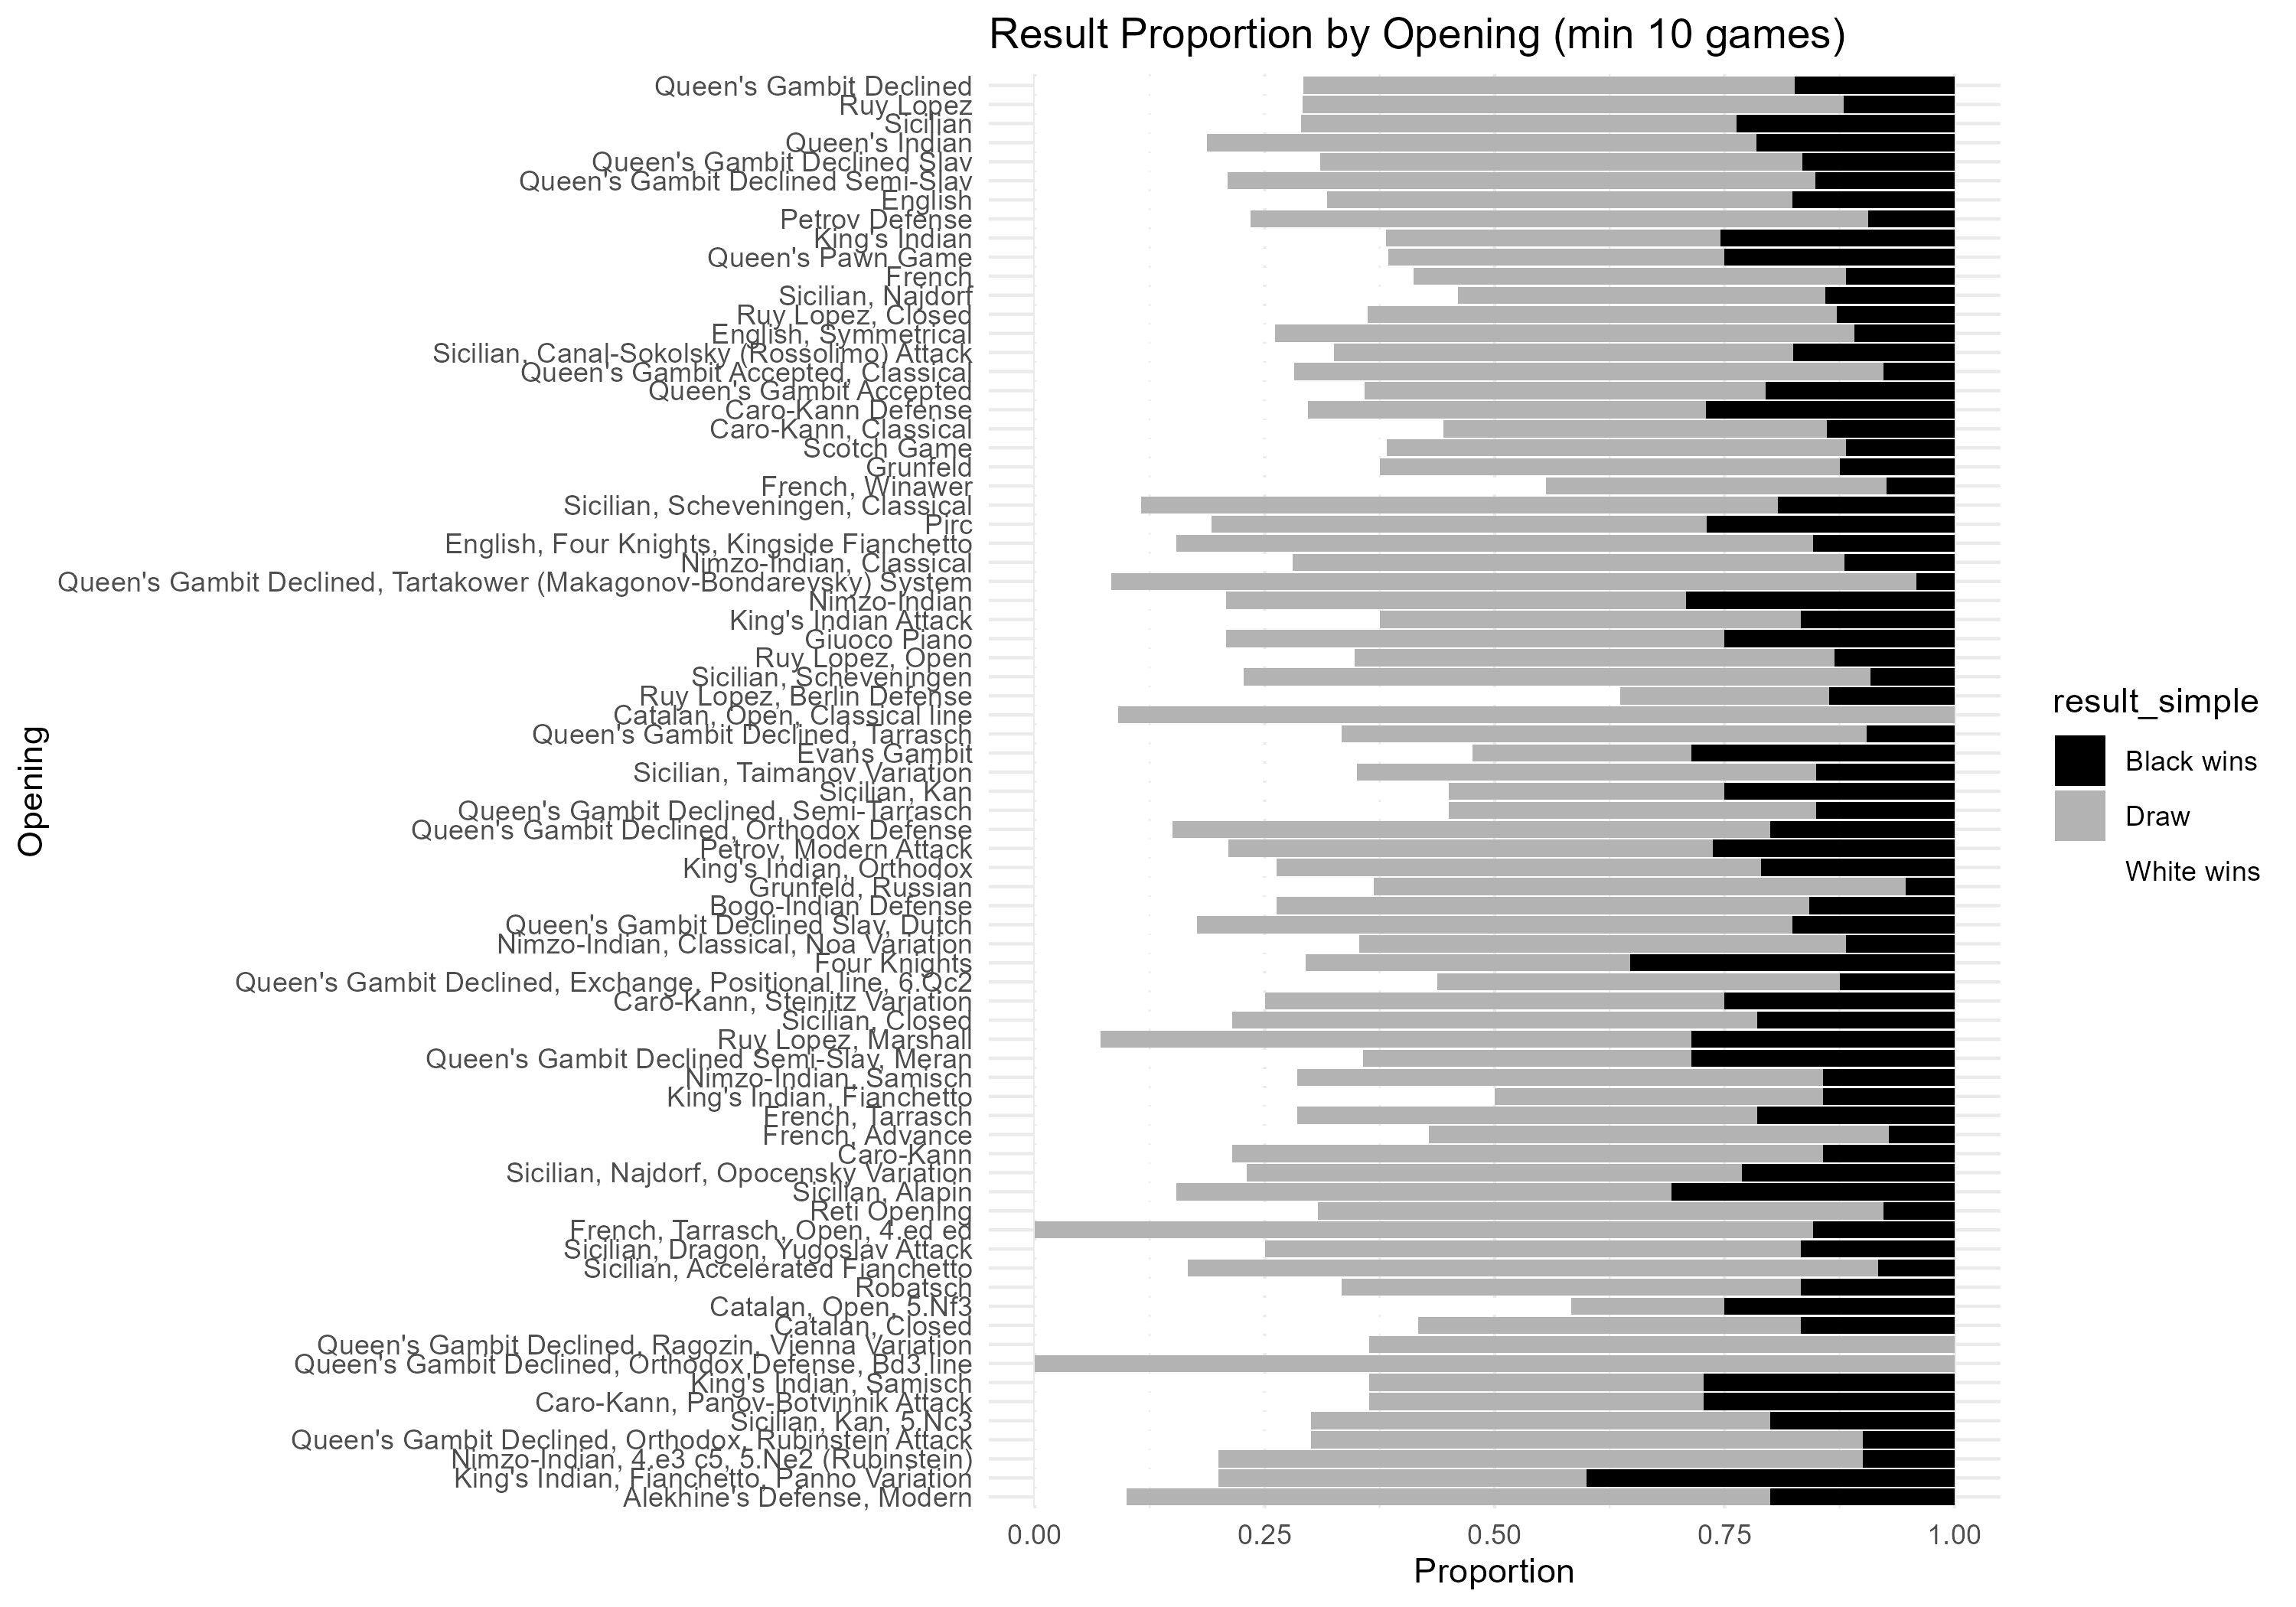
\includegraphics[width=0.9\textwidth]{../../ChessPlots/openings_by_result.png}
  \end{center}
  \small
  Proporcje wyników dla najpopularniejszych otwarć.
\end{frame}

\section{Otwarcia na przestrzeni dekad}
\begin{frame}{Grupy otwarć według dekady}
  \begin{center}
    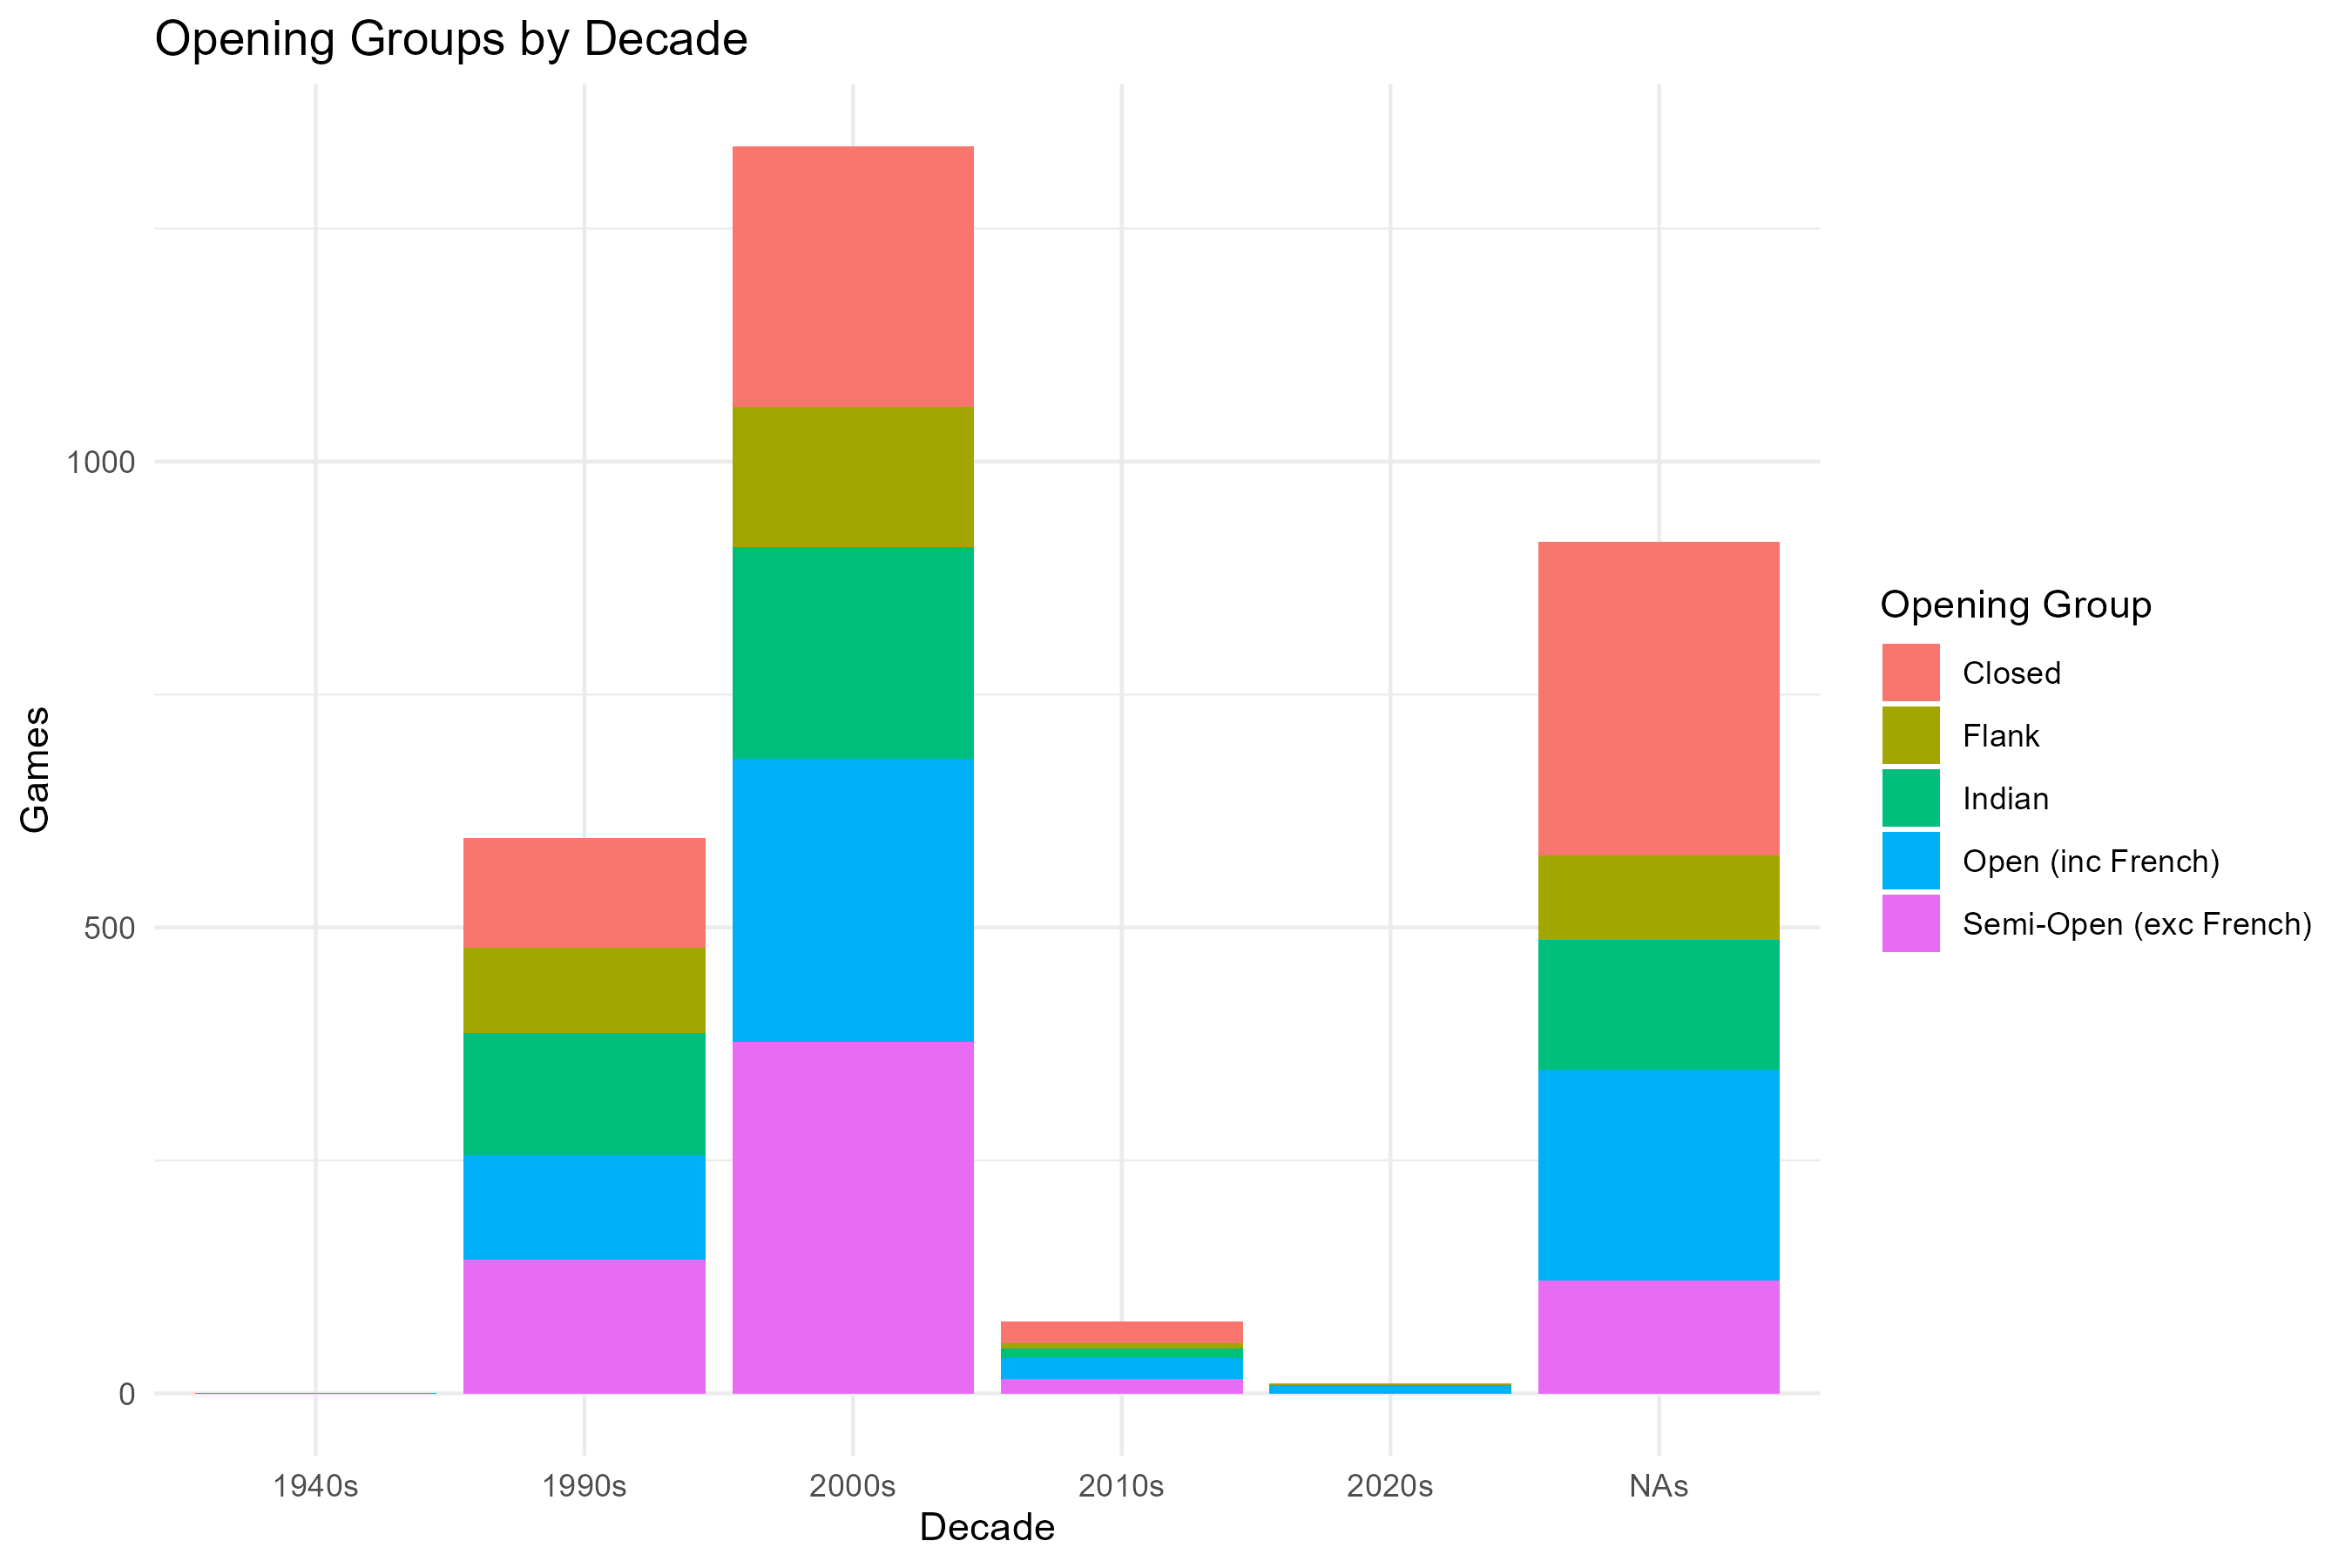
\includegraphics[width=0.8\textwidth]{../../ChessPlots/openings_by_decade.png}
  \end{center}
  \small
  Zmiany popularności grup otwarć w kolejnych dekadach.
\end{frame}

\section{Rankingi ELO w czasie}
\begin{frame}{Rankingi ELO zawodników na przestrzeni lat}
  \begin{center}
    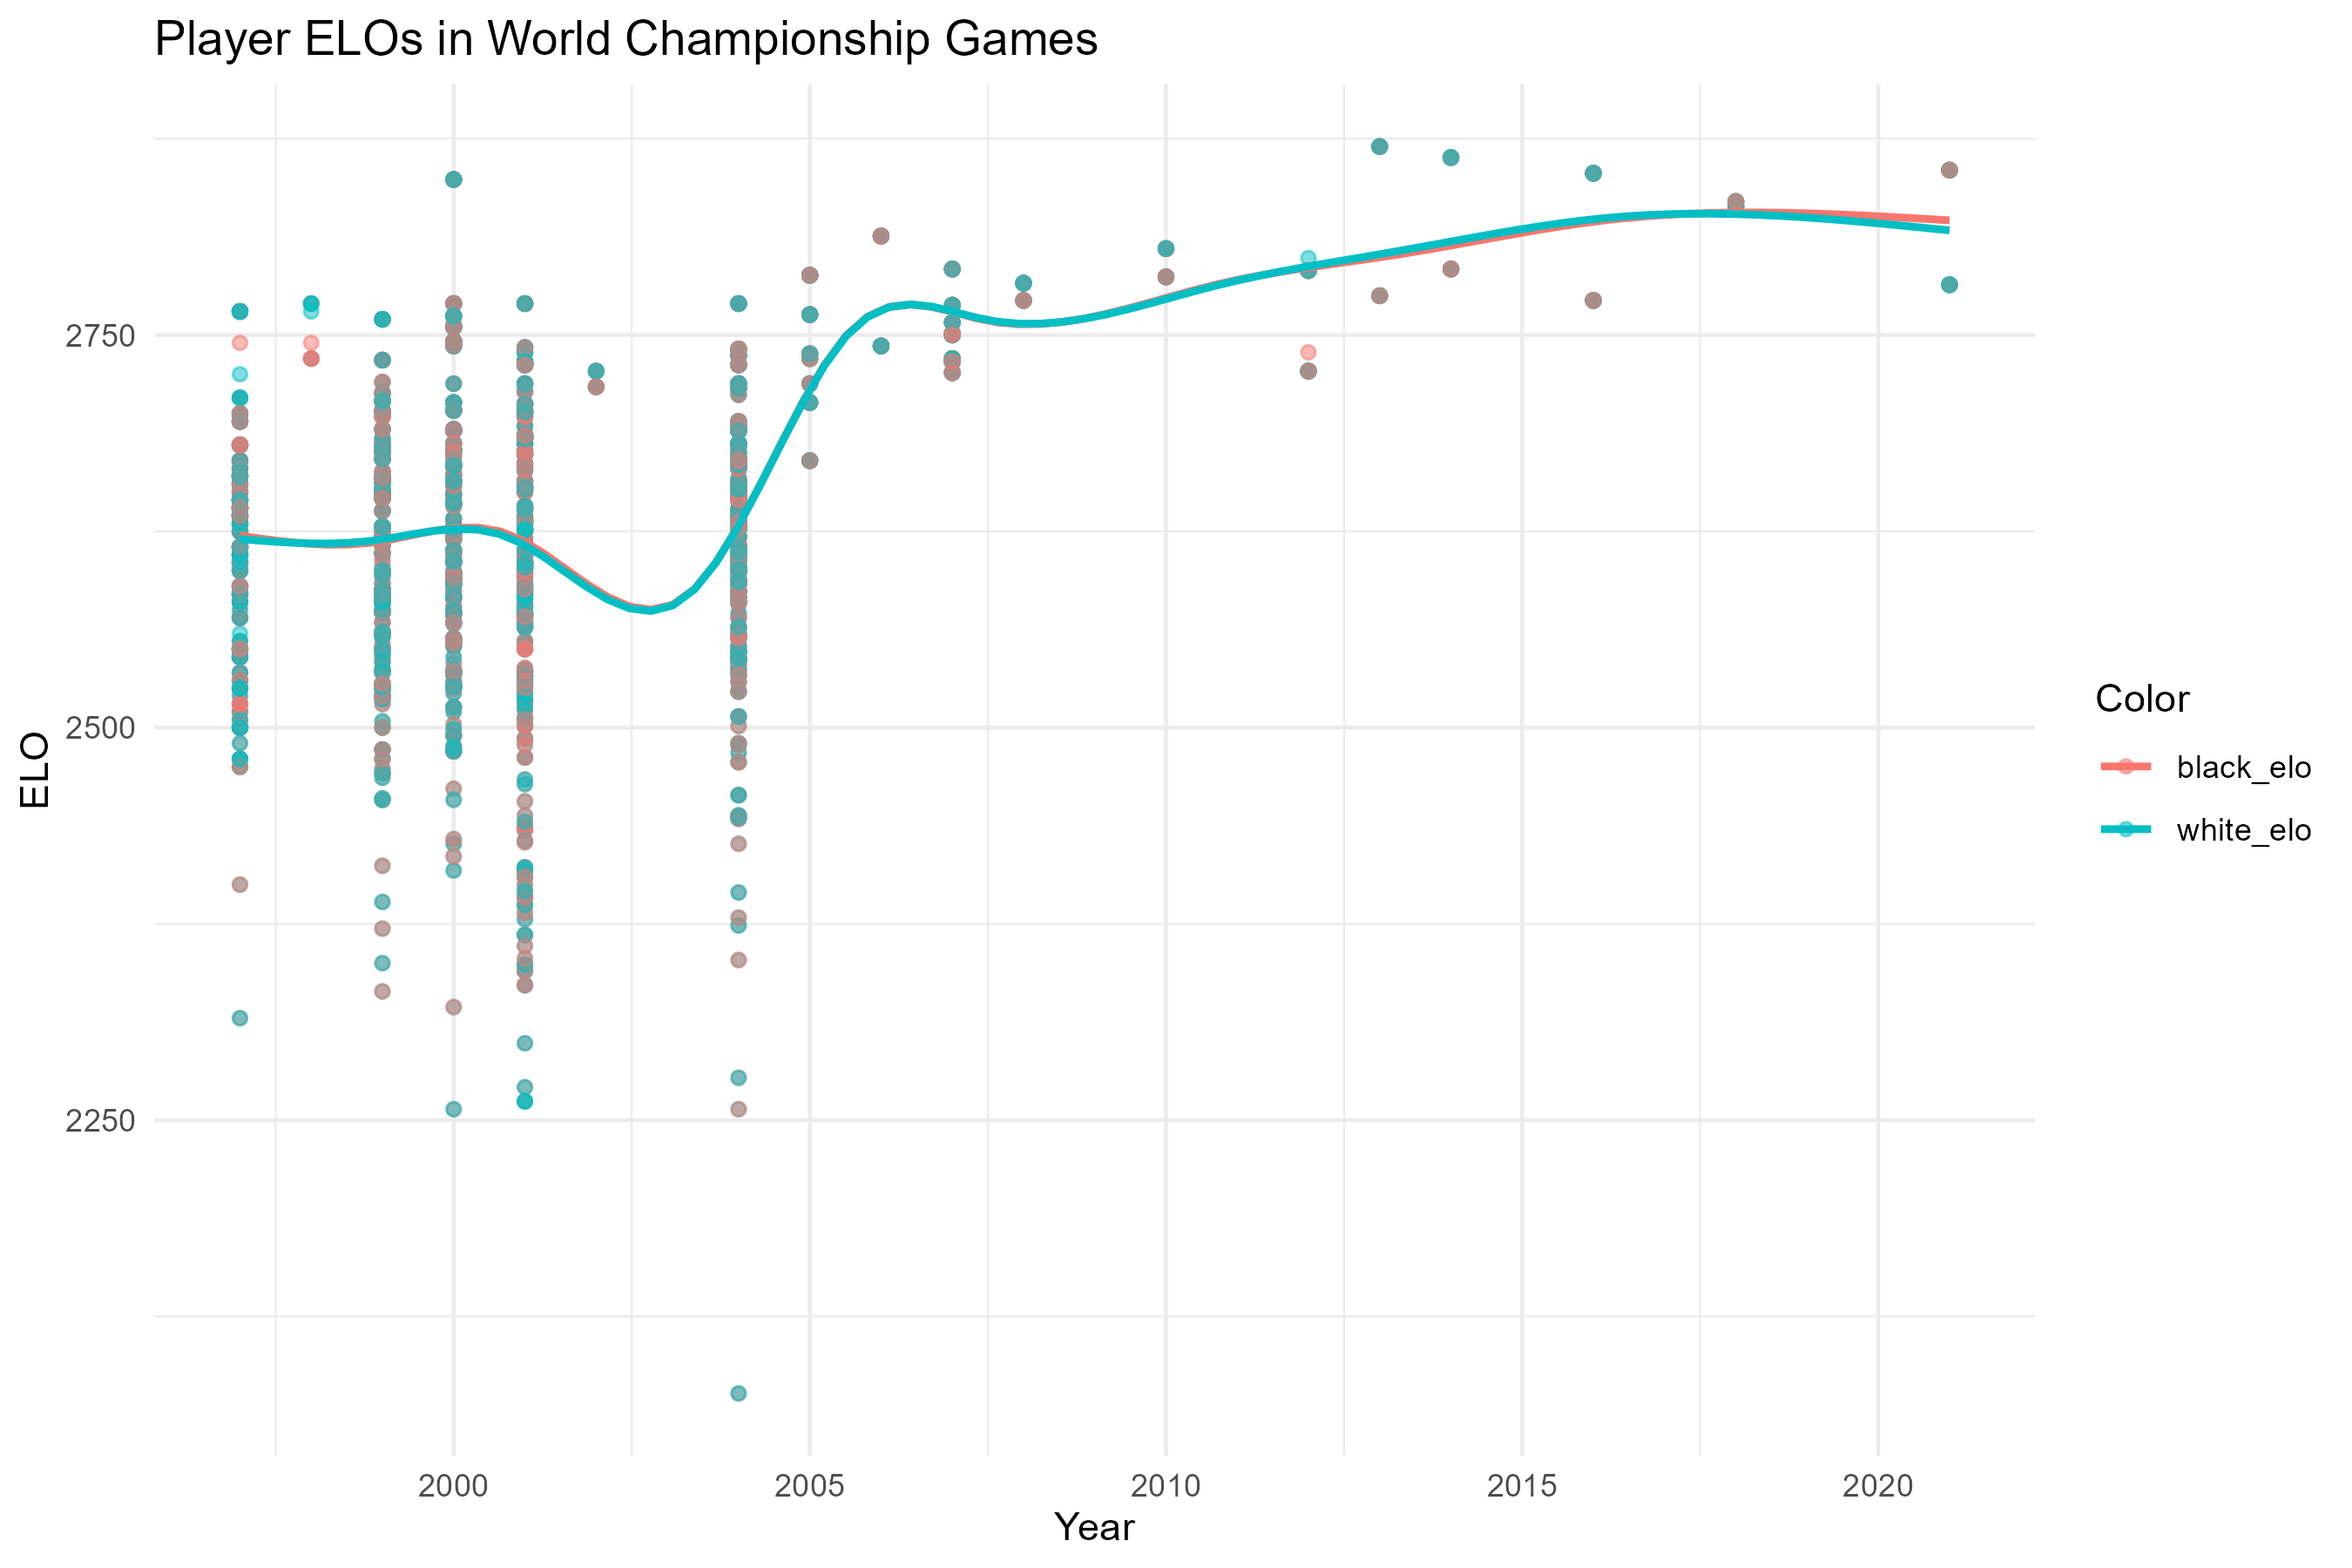
\includegraphics[width=0.8\textwidth]{../../ChessPlots/elos_over_time.png}
  \end{center}
  \small
  Zmiany rankingów ELO białych i czarnych w meczach o mistrzostwo świata.
\end{frame}

\section{Najczęściej grający zawodnicy}
\begin{frame}{Top 20 zawodników}
  \begin{center}
    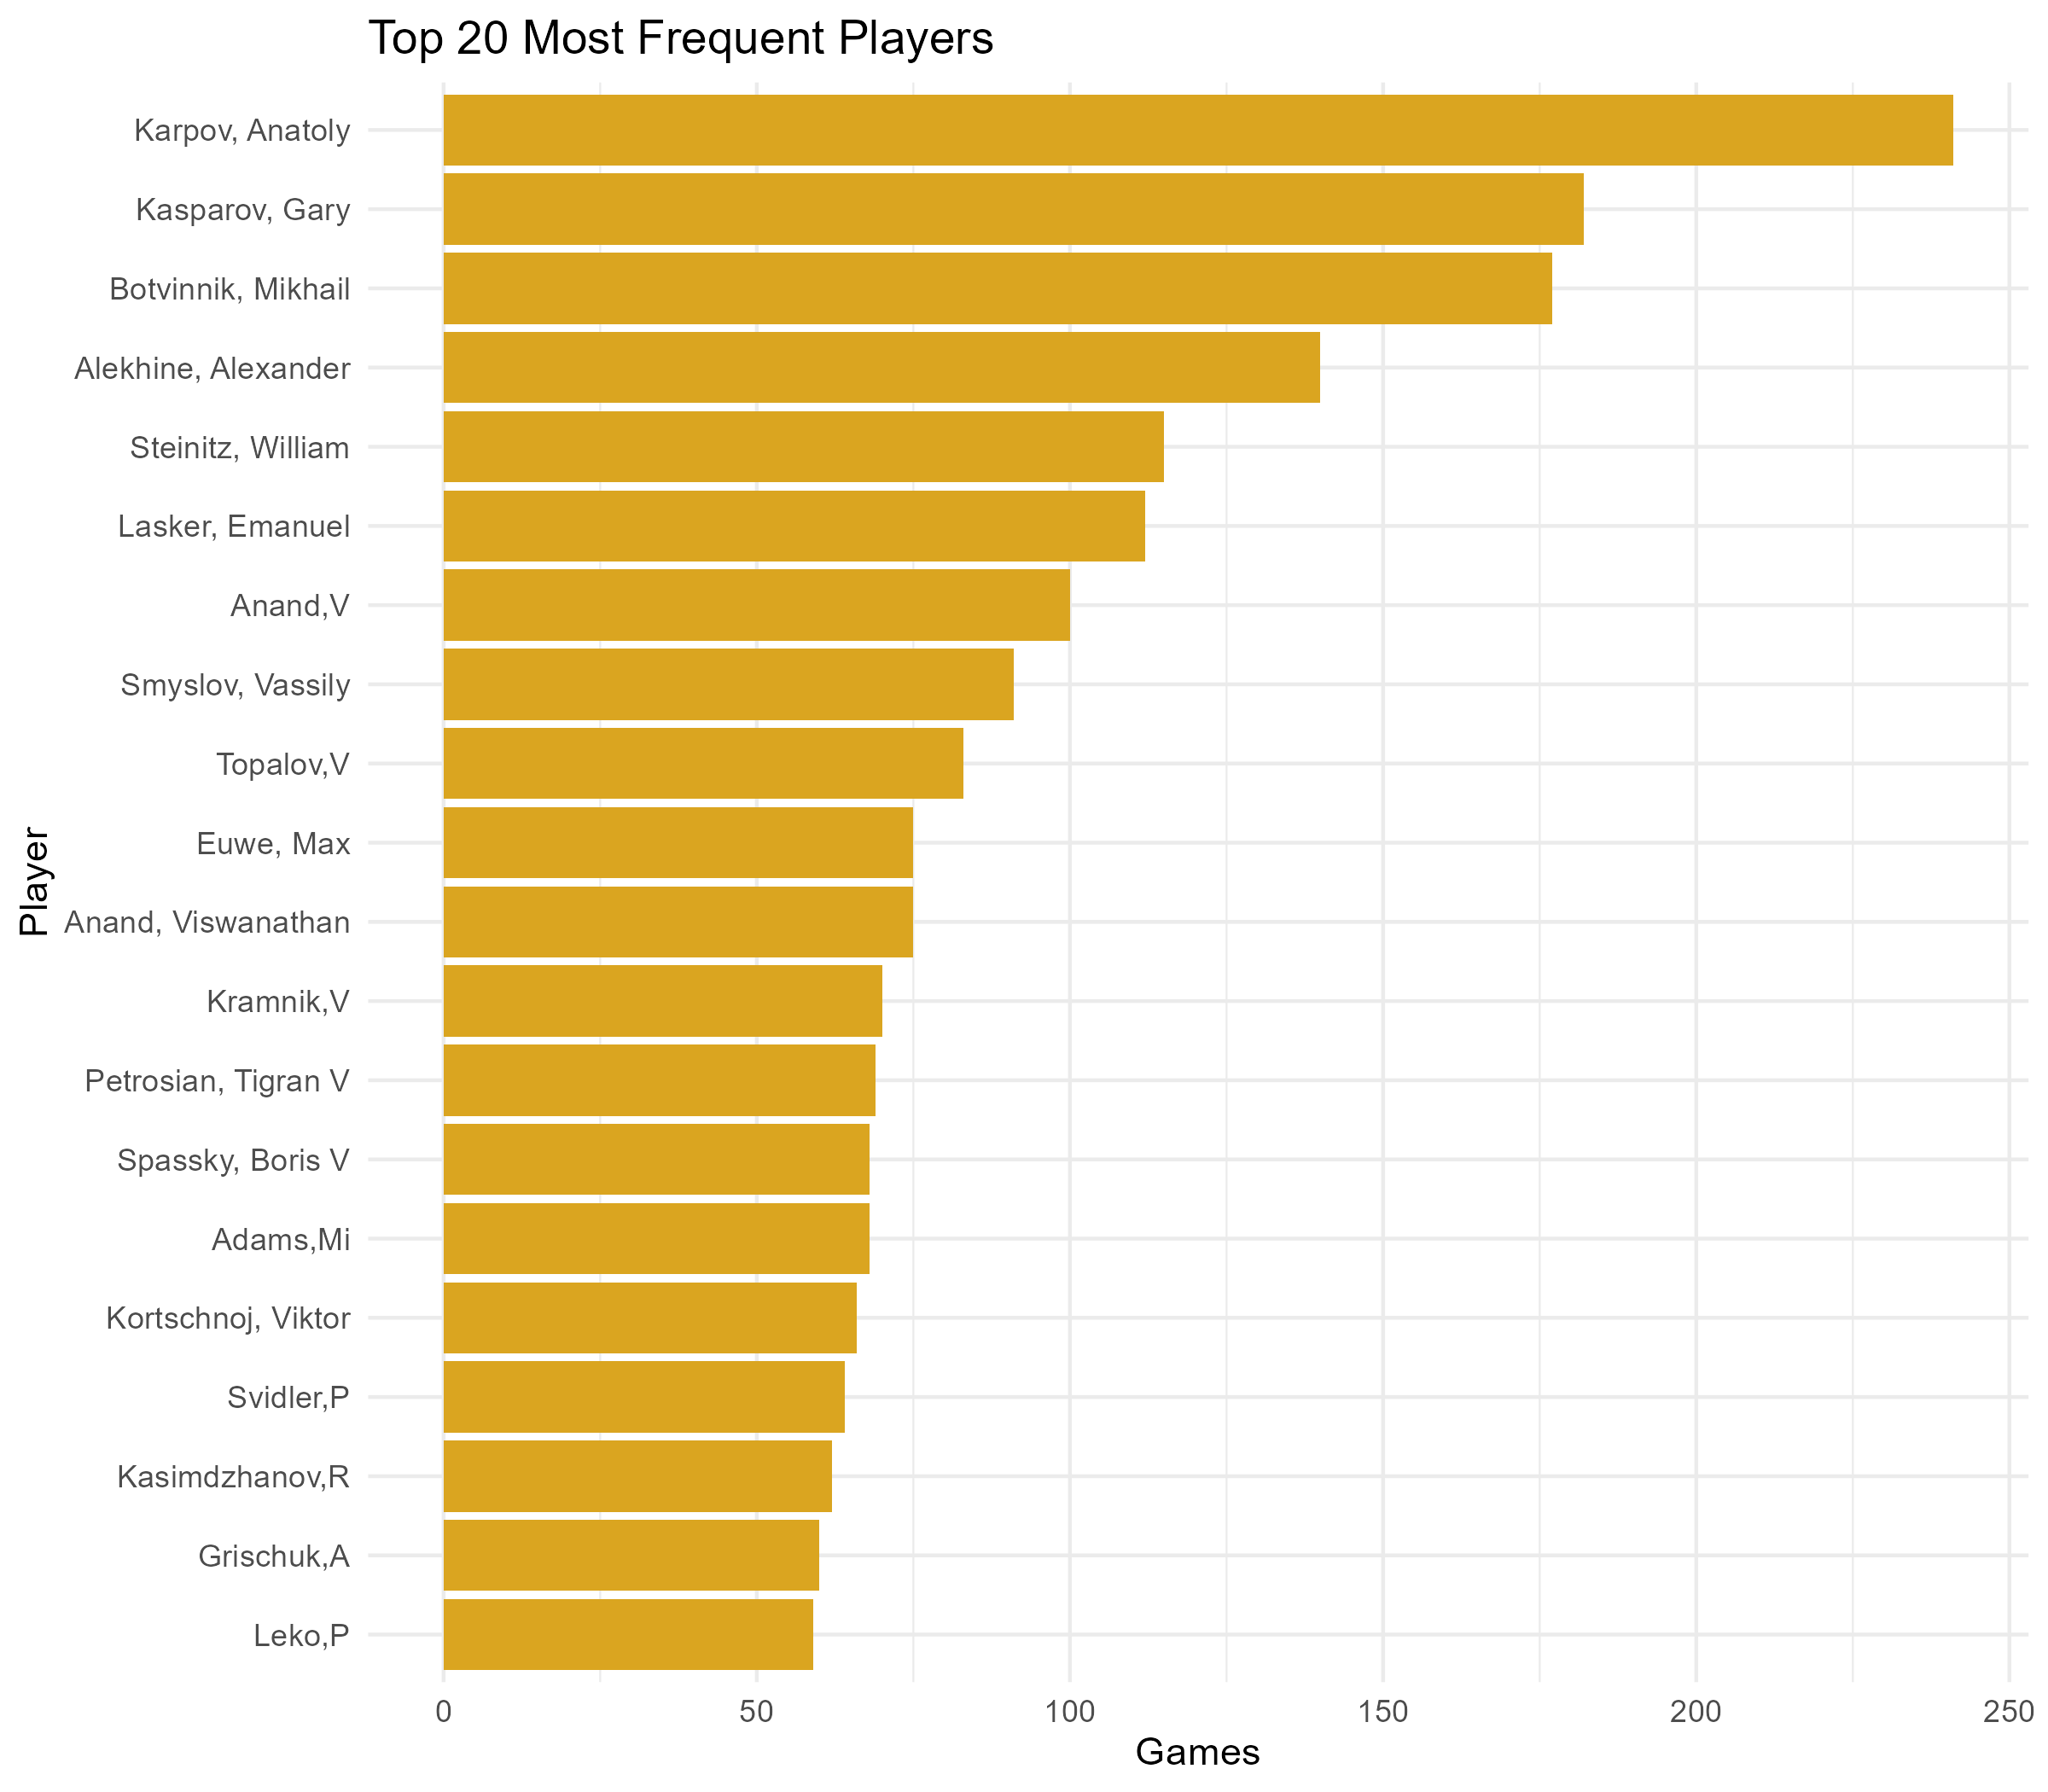
\includegraphics[width=0.8\textwidth]{../../ChessPlots/top20_players.png}
  \end{center}
  \small
  Zawodnicy z największą liczbą partii w historii mistrzostw świata.
\end{frame}

\section{Wyniki na przestrzeni lat}
\begin{frame}{Wyniki partii w czasie}
  \begin{center}
    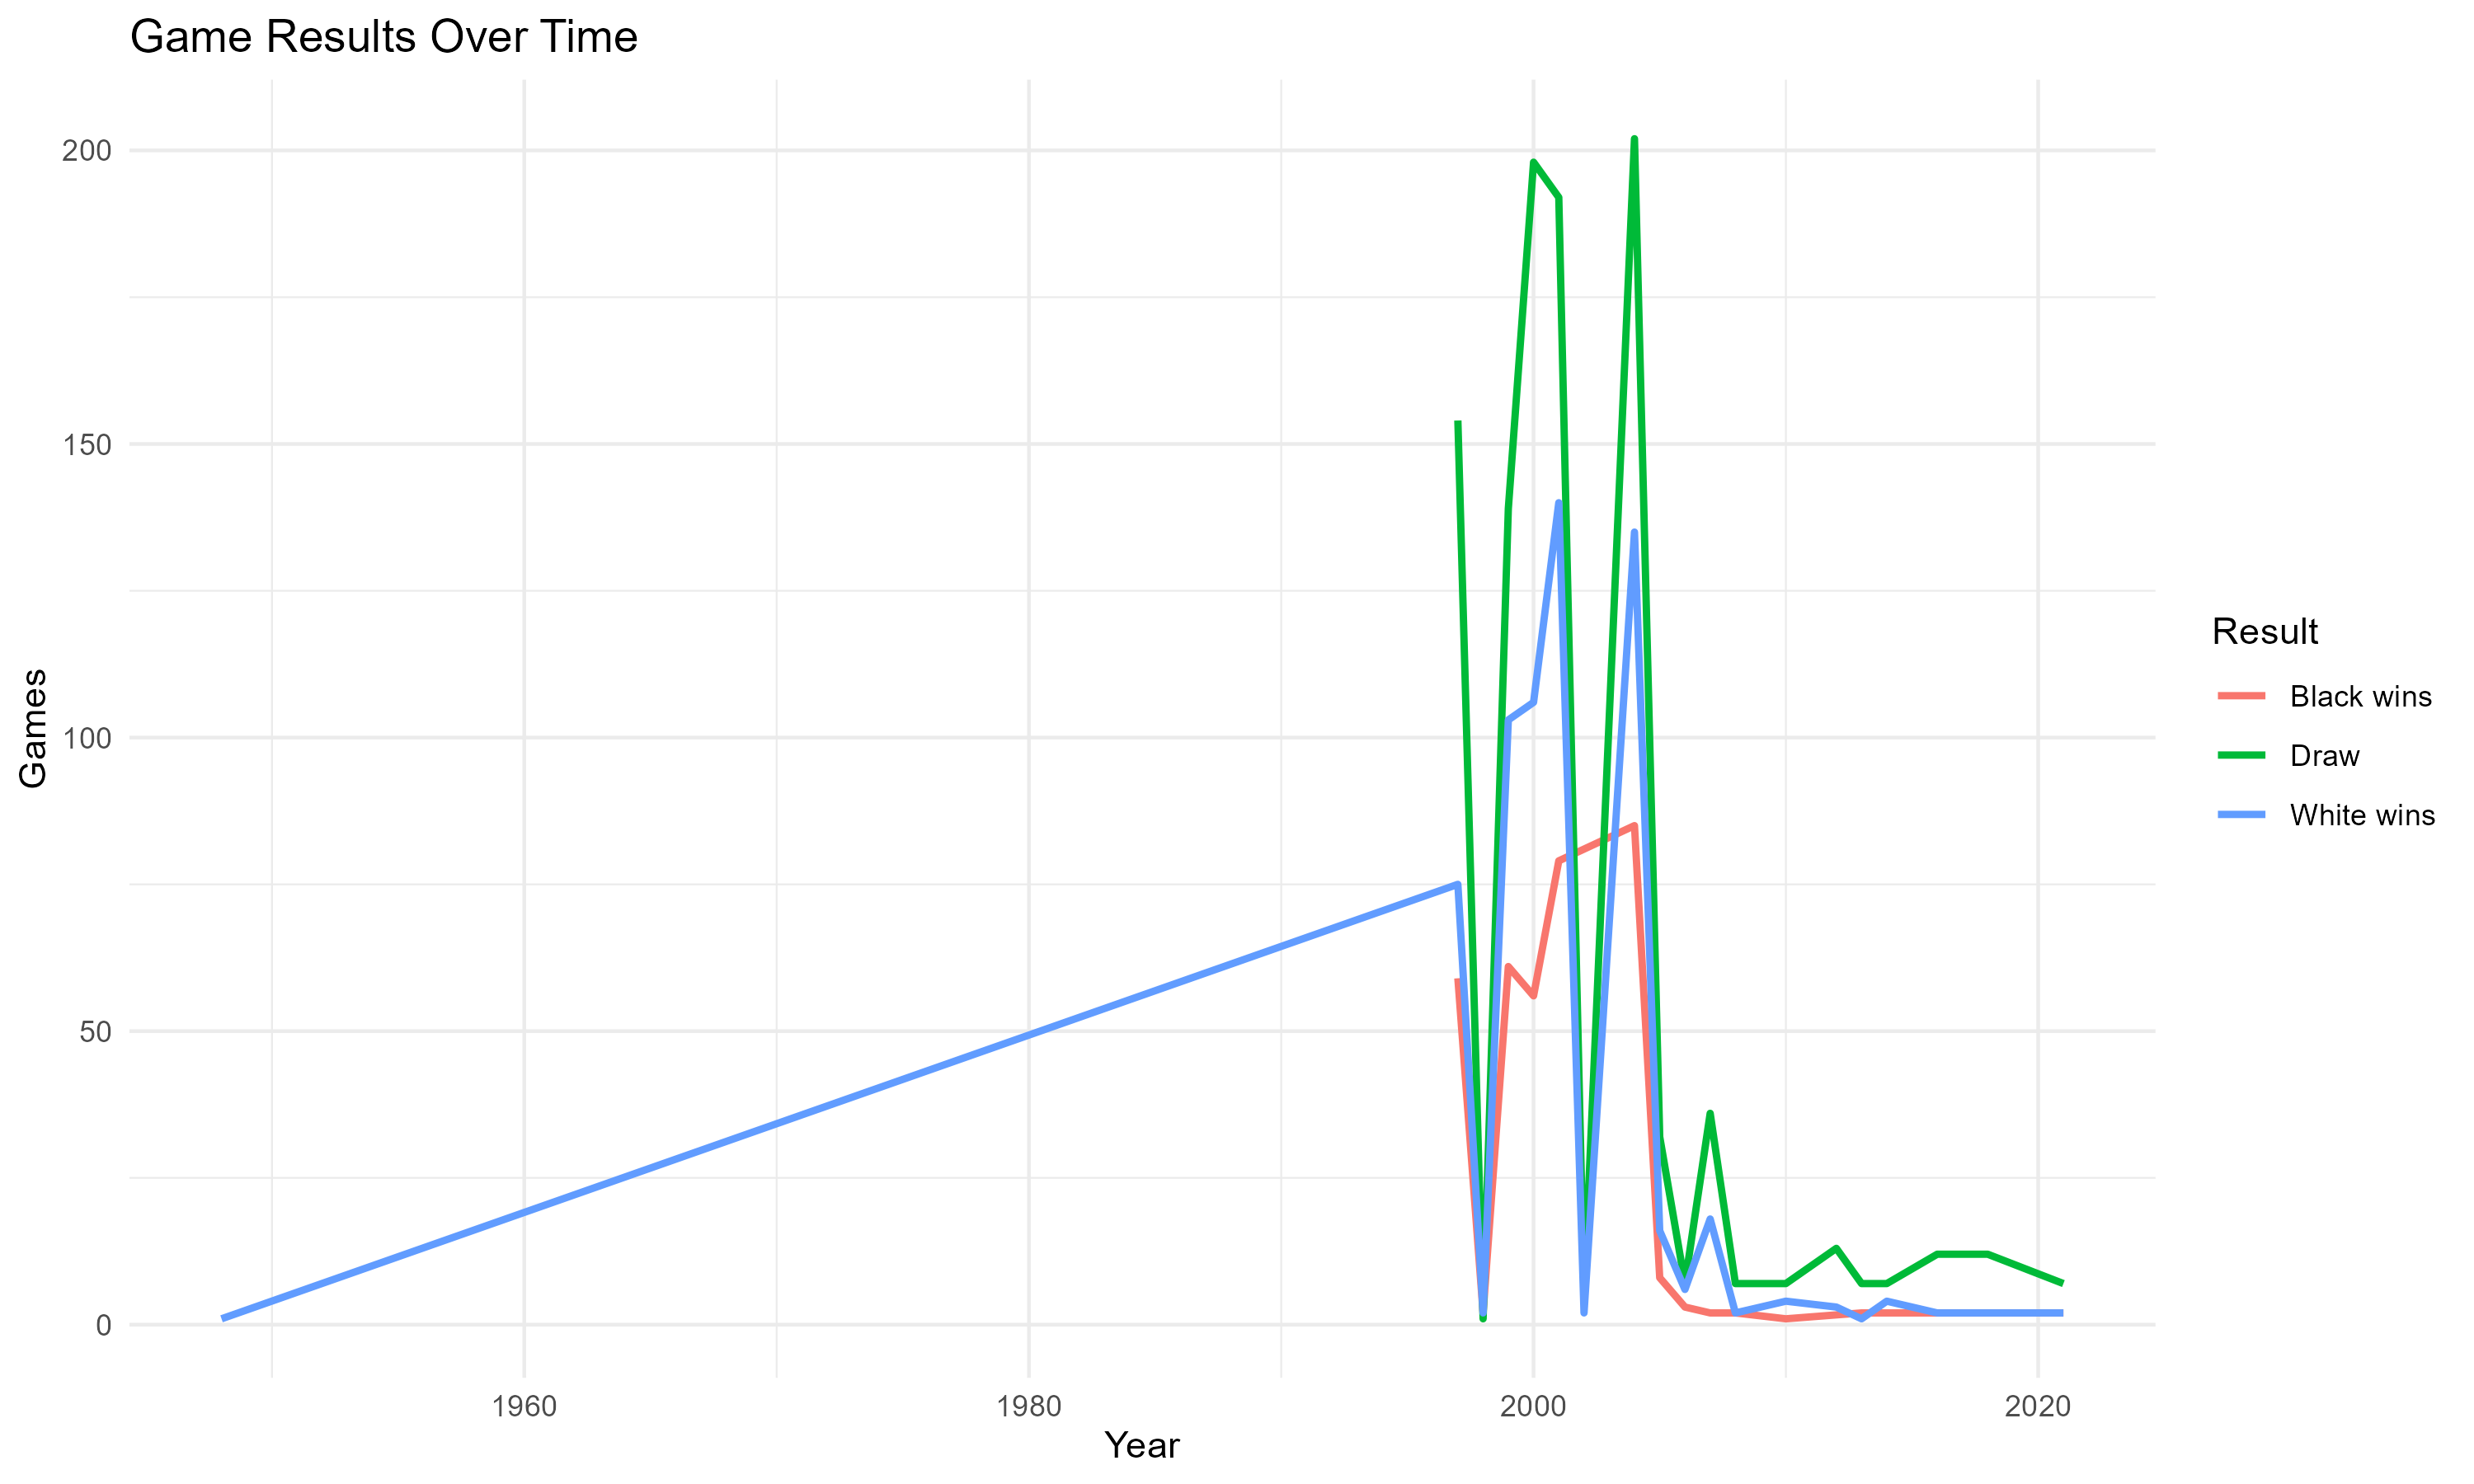
\includegraphics[width=0.9\textwidth]{../../ChessPlots/results_over_time.png}
  \end{center}
  \small
  Liczba zwycięstw białych, czarnych i remisów w kolejnych latach.
\end{frame}

\section{Podsumowanie}
\begin{frame}{Podsumowanie}
  \begin{itemize}
    \item Analiza pokazuje zmiany w popularności otwarć i wyników na przestrzeni lat.
    \item Widać dominację remisów w nowoczesnych meczach o mistrzostwo świata.
    \item Najlepsi zawodnicy często pojawiają się w czołówce statystyk.
  \end{itemize}
\end{frame}

\end{document}